% !TEX root = ../ClassicThesis_DEIB.tex

\chapter{Background and Tools} \label{chap:backgroundAndToolsChapter}

In this chapter we are going to describe the general concepts this thesis deals with, together with the main tools we used to address the project. Since this thesis is in the frame of \ac{GRAPE} project (see Chapter \ref{chap:grapeProject}),  most of them are typical of the robotic field and, more specifically, of the agricultural robotics. This last field should be seen in the wider context of the so-called \textit{E-agriculture}; to give a precise definition of this term, we make reference to the FAO (Food and Agriculture Organization) definition\footnote{http://www.fao.org/fileadmin/templates/rap/files/uploads/E-agriculture\_Solutions\_Forum.pdf}:
\blockquote{\textit{E-agriculture, or ICTs in agriculture, is about designing,
developing and applying innovative ways to use ICTs with a
primary focus on agriculture. E-agriculture offers a wide range
of solutions to agricultural challenges and has great potential
in promoting sustainable agriculture while protecting the
environment.}}
The \ac{GRAPE} project, that will be described with further details in chapter \ref{chap:grapeProject}, is about the design and realization of an \ac{UGV} with control and operative task in a vineyard environment, so in this chapter we'll deal with topics concerning software development in robotics, estimation of the state of a robot, autonomous navigation

%%%%%%%%%%%%%%%%%%%%%%%%%%%%%%%%%%%%%%%%%%%%%

\section{Robot Operating System}\label{sec:robotOperatingSystem}
\ac{ROS} is the \textit{robotic middleware} we used to develop the sofware components of the system described in this thesis. We decide to use it because of its great modularity, the availability of a very large number of packages, well documented APIs and an active community. Moreover, \ac{ROS} is a very widespread system, so its power and versatility are well known in the field of software development for robotics. Citing words from its offical website\footnote{http://wiki.ros.org/ROS/Introduction},
these are \ac{ROS} main features: 
\blockquote{
\textit{It provides the services you would expect from an operating system, including hardware abstraction, low-level device control, implementation of commonly-used functionality, message-passing between processes, and package management. It also provides tools and libraries for obtaining, building, writing, and running code across multiple computers}.
} 

\ac{ROS} is actually a \textit{meta-operating system}, that is, it's not an operating system in the traditional sense (it requires to be run on top of an another operating system; currently, the only officially supported OS is Linux Ubuntu), but it provides a peer-to-peer network that processes can use to create and process data together. This network is implemented through TCP, and it's called \textit{Computation Graph}. In this section, we're going to describe \ac{ROS} with more detail, with particular emphasis on the different tecniques that nodes can use to communicate among them. Keep in mind that, even if these tecniques differs a lot, they all are strongly typed \textit{i.e.} in order to define a channel (with \textit{channel} we now mean one of the tecnique that we are going to describe. It's not the name of a specific communication tool) you also need to define the types of message that are going to be exchanged throught it. \ac{ROS} already defines a lot of useful message types (\textit{e.g.} \textit{LaserScan.msg}, \textit{PoseWithCovarianceStamped.msg}), grouped by domain (\textit{e.g.}, \textit{Sensor\_msgs}, \textit{Geometry\_msgs}). However a simple message definition language is provided, and users are encouraged to define their own message types to make them as self-explanatory as possible.
\begin{description}
\item[ROS Master] Even if the Computation Graph is a peer-to-peer network, a central process, called  \textbf{\ac{ROS} Master}, is required to exist, to provide naming and registration services to all the user processes In this. Once the processes have located each other through the services offered by the Master, they can communicate peer-to-peer without involving a central entity;

\item[nodes] The processes that are in the Computation Graph are called \textbf{nodes}, and they are the atomic units of the computational graph. The \ac{ROS} API are available in C++, Python and Lisp, but C++ is the most widely used. One of the aims of \ac{ROS} is to be modular at a fine-grained scale, so a complex task should be achieved through cooperation of several different nodes, each with quite narrow tasks, rather than one large node that include all the functionalities. Nodes can use different techniques for communication, depending whether the message is a part of data stream or it is a request message (\textit{i.e.} a response message is expected) and, in this last case, on the (expected) duration and complexity of the computation of the response.

\item[topics] Topics implements a \textit{publish-subscribe} paradigm, are they the easiest way that nodes can use to communicate with each other, and basically are named channels, characterized by the type of the messages that are sent through it. When a node \textit{publish} a message on a certain topic, the message is read from all the nodes that previously \textit{subscribed} to that topic, interfacing with the Master. Note that:
\begin{itemize}
	\item this technique leads to a strong decoupling between publishers and subscribers to a topic, because a publisher node is, from an high-level perspective\footnote{Actually, publisher nodes always know the list of nodes subscribed to their topics. But this  is only used in connection phase, and to avoid a situation where a node publish on a topic with no subscribers, for the sake of efficiency.},
	not even aware of the presence of subscribers, and viceversa.
	\item the relationship between publishers and subscribers is \textit{many-to-many}, \textit{i.e.} multiple nodes can publish on a topic, and multiple nodes can subscribe to a topic.
\end{itemize}
We can easily conclude that this method is very suitable for passing streams of data (\textit{e.g.} the handler of a \ac{LIDAR} streams its measurements over the network, or a node publish the velocities commands for the wheels of a robot), but there is no notion of a \textit{response} to a message, so it's not suitable for \textit{request-response} communication. 

\begin{figure}
	\centering
	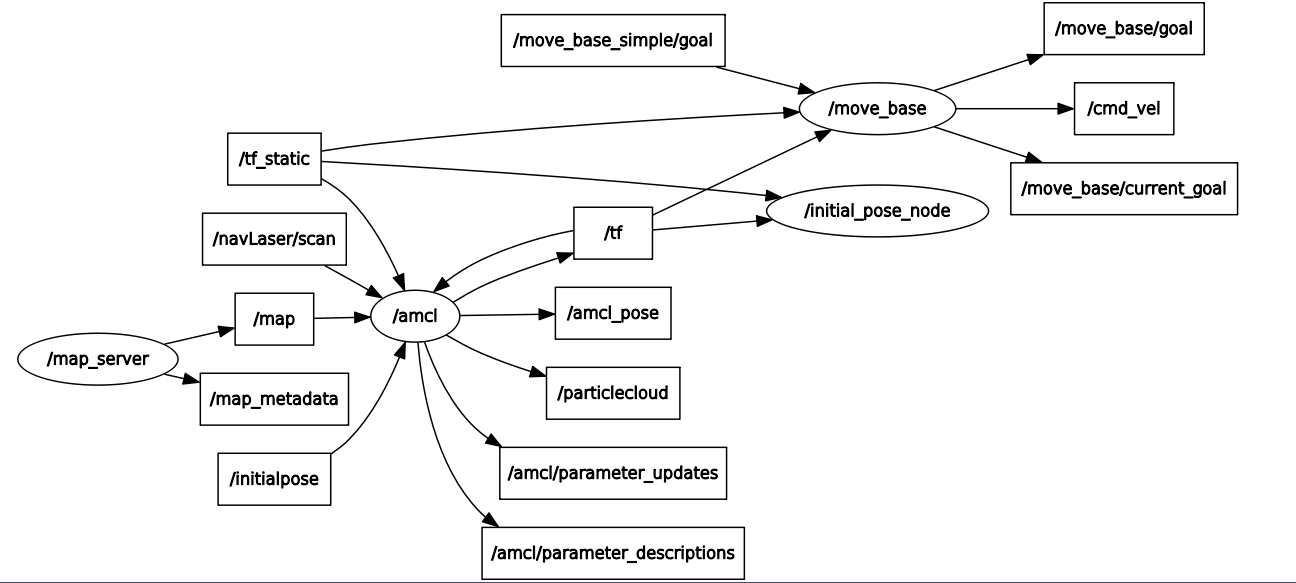
\includegraphics[width=1.1\textwidth]{Images/background_and_tools/rqt_graph.png}
	\caption{\textit{An example of the \ac{ROS} Computation Graph, visualized with} rqt\textit{: nodes are represented with circles, rectangles represent topics, and arrows go from a node to a topic it publishes on, or from a topic to a node subscribed to it. It's easy to recognize the} many-to-many \textit{relationship.}}
	\label{fig:tfGraph}
\end{figure}

\item[services] Services are defined by a name, and a couple of message types that describe the \textit{request} type and the \textit{response} type. Each service is offered by a Service server to any Service client that perform a call. So, Services implement an inter-node communication that is very similar to traditional function calling in most common programming languages (\textit{e.g.} C++, Java), in the sense that:
\begin{itemize}
	\item Service calls are blocking
	\item using Services, the inter-node communication is \textit{one-to-one}
\end{itemize}
These properties make Services suitable for punctual (in opposition to data stream) inter-node communication, such as: request of parameters values to another node, ask a node that handles a camera to take a picture, ask a node that perform navigation task to clear the current map.

\item[actions] While Services, with their resemblance to traditional function calls, can address pretty well the problem of \textit{one-to-one} inter-node communication, they can be quite unsatisfying if the computation required to produce the response is demanding in term of execution time (\textit{e.g.}, navigation of a robot from one point to another in an environment), because the caller is stuck at the line with the Service invocation until the end of the procedure. Services show their weaknesses also in situations where it could be useful to observe the intermediate results of the computation triggered by the request (\textit{e.g.}, a very complex manipulation procedure). \textbf{Actions} are very suitable in this context because, at the cost of a more complex implementation, provide an asynchronous and fully preemptable remote procedure call, with the possibility of monitoring intermediate results if needed. Differently from Topics and Services, Actions are not native in \ac{ROS}, and their functionalities are built on top of the other \ac{ROS} messagging systems. Asynchronicity is provided by the use of callbacks.
\end{description}

\begin{figure}
	\centering
	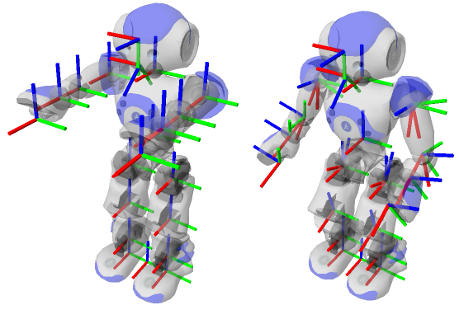
\includegraphics[width=0.8\textwidth]{Images/background_and_tools/tf_tree.png}
	\caption{\textit{A robot in 2 different positions, with} tf \textit{frames in evidence: x-axis is red, y-axis is green, z-axis is blue. The frames are the same in both configuration, but the transformations (i.e. rototranslations) between them are different.}}
	\label{fig:tfTreeRviz}
\end{figure}

%%%%%%%%%%%%%%%%%%%%%%%%%%%%%%%%%%%%%%%%%%%%%%

\section{TF: The Transform Library}\label{sec:tf}
\textit{tf} is a \ac{ROS} library, which task is very important to understand in order not to get lost in the next sections and chapters.  The goal of \textit{tf} is:

\blockquote{
\textit{" [...] provide a standard way to keep track of coordinate frames and transform data within an entire system such that individual component users can be confident that the data is in the coordinate frame that they want without requiring knowledge of all the coordinate
frames in the system" \parencite{tfPaper}}
}
The utility of such a component is straightforward, even in quite simple robotic systems. We'll describe here a situation we stumpled upon exactly in the development of the \ac{GRAPE} project, where of the utility of \textit{tf} is very easy to understand; you'll be able to better contextualize this example after you've read Chapter \ref{chap:kinovaArmChapter}. In this example a \ac{LIDAR}, mounted on top of the final joint of a robotic arm, acquires data while the arm is moving in order to create a point cloud that will be processed later. To get a meaningful point cloud, it's mandatory to keep track of the movement of the \ac{LIDAR} with respect to a point with speed equal to zero (\textit{e.g.} the base link of the arm, or the base link of the whole robot), and this gets even more difficult because of the multiple (6 in our specific case) joints of the arm; but this problem can be easily addressed by means of \textit{tf}, that we are now going to describe with more detail. 
\textit{tf} implementation relies on \ac{ROS} topics (see Section \ref{sec:robotOperatingSystem}) and achieves the goal mentioned before by building an oriented graph where vertices are reference frames, and edges are transformations (rototranslations) between frames. \textit{tf} does not assume a constant structure and, if a path exists between two reference frames in the graph, the direct transformation between them can be computed by composition of transformation. Since, in general, multiple paths between 2 vertices can exists in a directed graph and this could lead to ambiguity in computing the transformation between two reference frames, the graph is forced to be acyclic. Discongit anected subgraphs are allowed, but of course transformation between vertices that belong to different subgraphs cannot be computed. 
The main components of the library are:
\begin{itemize}
	\item \textbf{\textit{tf} broadcasters}: they are simple software components, that publish a transformation between two reference frames every time an update is available. Different broacasters does not sync together the publishing phase
	\item \textbf{\textit{tf} listeners}: they are more complex components, because they take into account that broadcasters are not synced. Since both transformations and queries to \textit{tf} graph are stamped, listeners make use of queues to store the most recent transformations, and they  interpulate old values using SLERP (Spherical Linear intERPolation) to return a transformation for which there is no measured value at the requested timestamp.
\end{itemize}

\begin{figure}
	\centering
	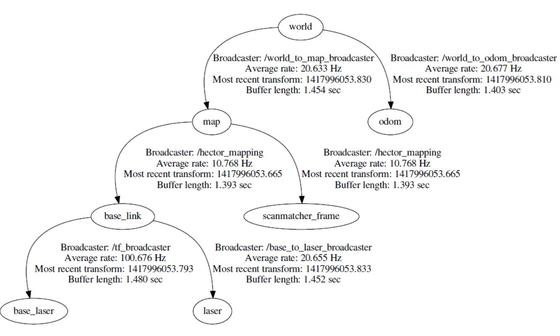
\includegraphics[width=0.6\textwidth]{Images/background_and_tools/tfGraph.JPG}
	\caption{\textit{An example of} tf \textit{tree}}
	\label{fig:tfGraph}
\end{figure}

In figure \ref{fig:tfTreeRviz} you can see a graphical representation of the reference frames tracked in a Nao Robot, while figure \ref{fig:tfGraph} shows an example of \textit{tf} graph visualized with visualization framework \textit{rqt}. 

%%%%%%%%%%%%%%%%%%%%%%%%%%%%%%%%%%%%%%%%%%%%%%%%%

\section{Odometry}\label{sec:odometry}

\begin{figure}
	\centering
	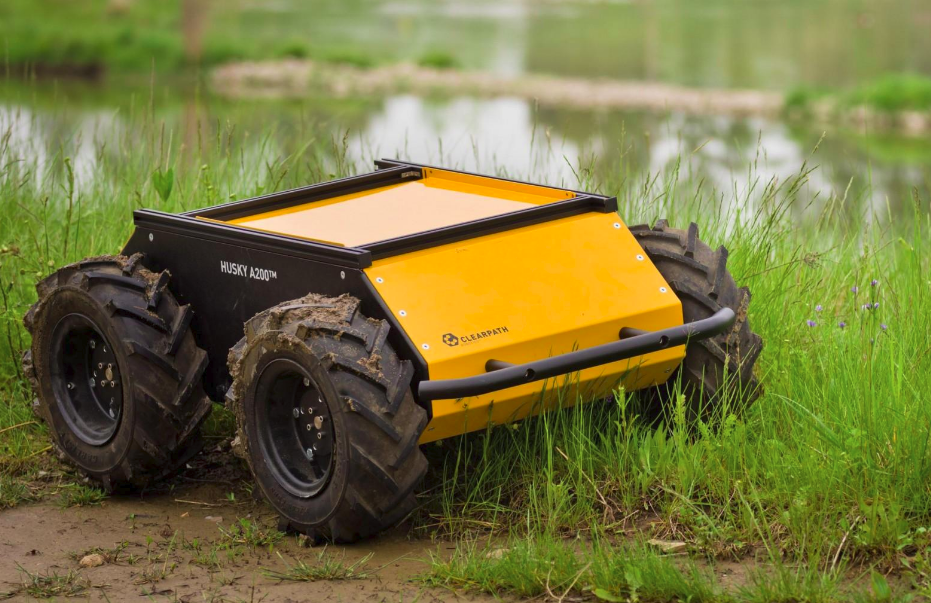
\includegraphics[width=0.6\textwidth]{Images/background_and_tools/husky.png}
	\caption{\textit{Husky platform from Clearpath Robotics is the platform used for the development of \ac{GRAPE} project.}}
	\label{fig:husky}
\end{figure}

The problem of odometry, \textit{i.e.} estimation of the position of a robot in an environment is harder than it could seem. Formally, odometry estimation is the problem of estimating over time the tuple: 
\begin{equation}
	<x, y, z, \theta,\dot{x}, \dot{y}, \dot{z}, \dot{\theta}>
	\label{eq:odometryTuple}
\end{equation} 
given the measurement of some motion sensors. 
To better understand the complexity of the problem, let's analyze an extremely simple model: a robot with a single, freely rotating wheel. In this frame, assuming rotary encoders on the wheel, we can think about measuring directly the wheel speed and integrate these measurement to get the travelled distance, and measure the variation in the orientation of the wheel to get the position. But actually there are a lot of imperfection that can lead to error, for example:
	\begin{itemize}
		\item wheel can be non perfectly perendicular to the ground
		\item the friction between the floor and the wheel might not be enough to avoid slippage (expecially )
		\item there is no such thing as a perfect sensor, so the use of encoders introduce an error
	\end{itemize}
Even if all these concurrent causes seem negligible, you have to take into account that the errors sum up over time, so an error of a few millimeters per meter might become significant over time. \\ 
Moreover, the probability of slippage gets higher in systems with more than one wheel, because, because for a system with multiple wheels to move without slippage, a point must exists around which all the wheels can move along a circular path. This point is called \ac{ICC} (see Figure \ref{fig:icc}), and can be easily identified by looking for the intersection of the axis of all wheels. If the intersaction exists in a single point, it's called the \ac{ICC}.
But even if the odometry estimated from the wheels is not a good solution if used alone, it can be used as a starting point for other, more complex, method. For this reason we are now going to descript how to estimate the odometry starting from the wheels encoders in our specific robot. This computation is different according to the \textbf{motion model} of the considered robot. As we'll see in Section \ref{sec:grapeHwArch}, the robot we used is the Husky platform (see Figure \ref{fig:husky}) from Clearpath Robotics, that moves with a  \textit{skid steering} kinematics, that is a derivative of \textit{differential drive} kinematics. Thus, we're going to describe these two motion model with more detail.


\begin{figure}
	\centering
	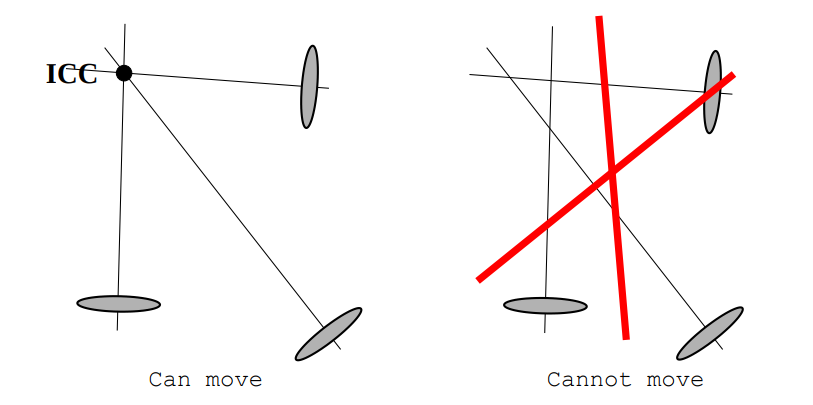
\includegraphics[width=0.8\textwidth]{Images/background_and_tools/icc.png}
	\caption{\textit{If the axis of all the wheels intersect in a single point, it's called ICC and the robot can move without slipping}}
	\label{fig:icc}
\end{figure}

\subsection{Differential drive robot}
In a differential drive system, the movement of the robot is only based on two separately driven wheels, placed on either side of the robot, on the same axis (see Figure \ref{fig:diffDrive}), and optionally a central, non-actuated caster wheel for stability. The two side wheels are not steerable, so the changes of direction are realized through application of different speed to the two wheels. For example, intuitively, if the wheels move at the same speed and in the same direction, the robot will move straight; if the wheels move at the same speed but different directions, the robot rotates in place.
 By recalling the definition of \ac{ICC}, we observe that, if the wheels are correctly aligned, a differential drive robot always have a well-defined \ac{ICC} and the slippage of the wheels is not very accentuated. \\
At each instant in time, since the \ac{ICC} is well-defined, both the left and right wheel follow a path that moves around \ac{ICC} at the same angular speed $\omega$, and thus:

\begin{empheq}[left=\empheqlbrace]{align}
\omega (R + \frac{L}{2}) = v_r  \label{eq:diffDrive1}\\ 
\omega (R - \frac{L}{2}) = v_l   \label{eq:diffDrive2}
\end{empheq}

where $L$ is the distance between the center of the two wheels, $v_r$ and $v_l$ are, respectively, the linear velocity of the right and left wheel, $R$ is the signed distance between the \ac{ICC} and the midpoint of the wheels. Note that the only parameter constant through time is $L$, since it's a physical property of the robot structure, while all other parameter evolve during the movement. \\
By combining \ref{eq:diffDrive1} and \ref{eq:diffDrive2}, we get:

\begin{empheq} {align}
R=\frac{L}{2} \frac{(v_r+v_l)}{(v_r-v_l)},  \qquad \omega=\frac{(v_r-v_l)}{L}
\end{empheq}

Observing these results we can validate the intuitive impressions about particular cases made a few lines above:
\begin{itemize}
	\item if $v_r=v_l$, the curvature radius is infinite, because the robot is moving straight.
	\item if $v_r=-v_l$, the robot is moving around the midpoint of the wheels
\end{itemize}
We give now some details about odometry computation. Let's assume, in a certain moment $t=t_0$, that the robot pose is $(x,y,\theta)$. We assume that in the time interval $t_0\rightarrow (t_0 +\delta t$) the values $v_r$ and $v_l$ are constant; if we observe figure \ref{fig:diffDriveDeltaT} under these condition, we have:
\begin{equation}
	ICC=(x-Rsin\theta, y+Rcos\theta)
\end{equation}
Write now the expressions for $(x',y',\theta')$:

\[
\begin{bmatrix}
\dot{x} \\
\dot{y} \\
\dot{\theta}
\end{bmatrix}
 = 
\begin{bmatrix}
cos(\omega \delta t) & -sin(\omega \delta t) & 0 \\
sin(\omega \delta t)  & cos(\omega \delta t) & 0 \\
0                                       & 0                                      & 1
\end{bmatrix}
\begin{bmatrix}
x-ICC_x\\
y-ICC _y\\
\theta
\end{bmatrix}
+
\begin{bmatrix}
ICC_x \\
ICC_y \\
\omega \delta t
\end{bmatrix}
\]

With this procedure we have identified 3 of the elements of the target tuple (see expression \ref{eq:odometryTuple}), but we still have to retrieve $x$,$y$ and $\theta$. For this reason we consider that by assuming an initial pose ($x_0, y_0, \theta_0$), knowing that:
\begin{equation}
	V(t)=\frac{(v_r+v_l)}{2}
\end{equation}
where $V(t)$ represent the complexive speed of the robot, and assuming to know the functions $v_r(t)$ and $v_l(t)$ \textit{i.e.} the linear speed of the wheel in time, we can calculate $(x,y,\theta)$ by integrating the speed of the robot over time, that is:

\begin{empheq}{align}
	x(t)            & = \int_{0}^{t}V(t)cos(\theta(t))dt \\
	y(t)            & = \int_{0}^{t}V(t)sin(\theta(t))dt \\
	\theta(t)  & = \int_{0}^{t}\omega(t)d\omega
\end{empheq}

and, in our specific case we can write it as function of $v_l$ and $v_r$, that are the quantities that are directly measured on the wheels.

\begin{empheq}{align}
	x(t)            & = \frac{1}{2}\int_{0}^{t}(v_r(t)+v_l(t))cos(\theta(t))dt \\
	y(t)            & = \frac{1}{2}\int_{0}^{t}(v_r(t)+v_l(t))sin(\theta(t))dt \\
	\theta(t)  & =\frac{1}{L} \int_{0}^{t}(v_r(t)-v_l(t))(t)
\end{empheq}
So the tuple required by the odometry calculation is now complete.


\begin{figure}
	\centering
	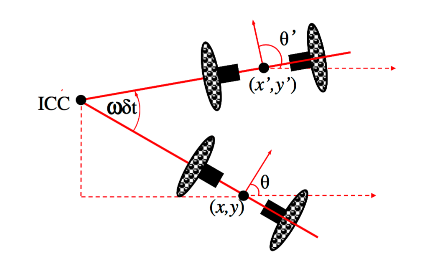
\includegraphics[width=0.8\textwidth]{Images/background_and_tools/diffDriveDeltaT.png}
	\caption{\textit{Differential drive: $(x,y,\theta) \rightarrow (x',y',\theta')$}}
	\label{fig:diffDriveDeltaT}
\end{figure}















\cleardoublepage
\begin{itemize}

	\item cosa si intende per odometria
	\item motion models: differential drive e skid steering
	\item sensor fusion cos'è, e esempio di Robot localization
	\item localizzazione con amcl
\end{itemize}
\begin{figure}
	\centering
	\subfloat[]{%
		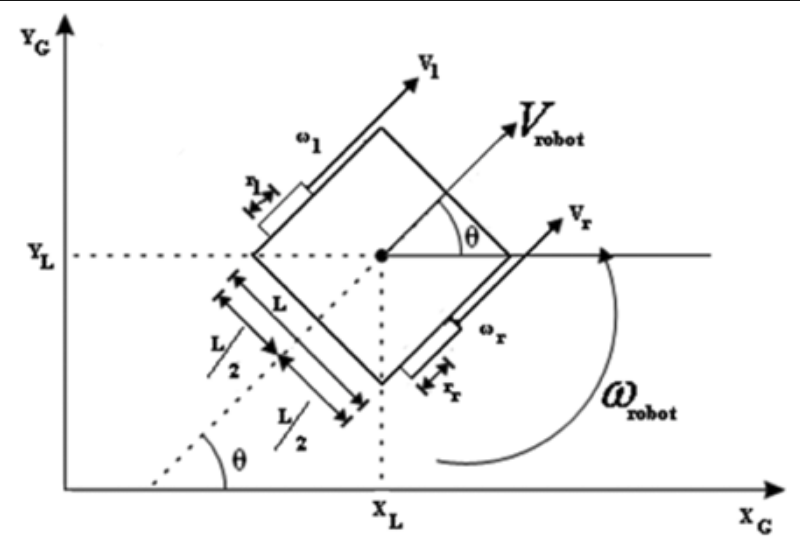
\includegraphics[width=0.55\textwidth]{Images/background_and_tools/diffDrive.png}
		\label{fig:diffDriveA}}
	\qquad
	\subfloat[]{%
		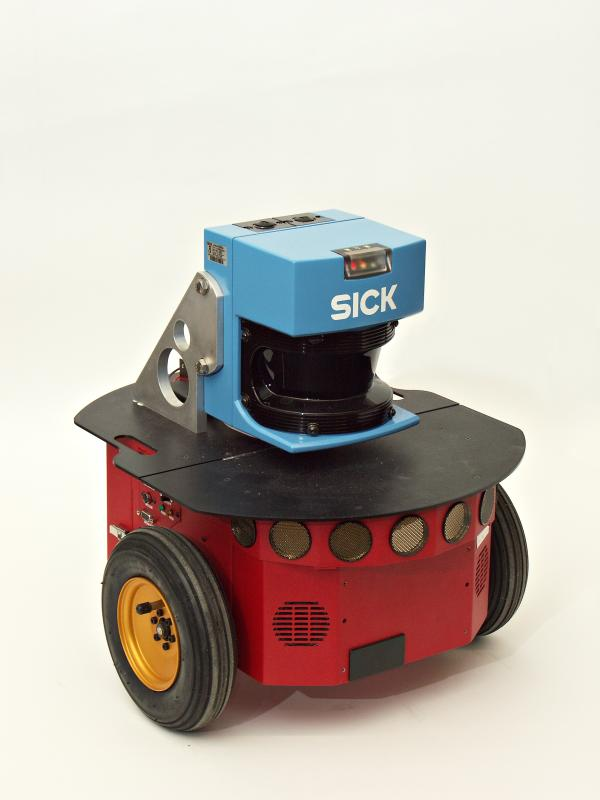
\includegraphics[width=0.3\textwidth]{Images/background_and_tools/diffDriveExample.jpg}
		\label{fig:diffDriveB}}
	\caption{\textit{On figure \ref{fig:diffDriveA}, the scheme of a differential drive motion model; in figure \ref{fig:diffDriveB}, an example of a differential drive robot (Pioneer 3DX).}}
	\label{fig:diffDrive}
\end{figure}

%%%%%%%%%%%%%%%%%%%%%%%%%%%%%%%%%%%%%%%%%%%%%%%%

\section{Navigation Stack}\label{sec:navigationStack}
SKETCH:
\begin{itemize}
	\item cos'è navigation stack (immagine http://wiki.ros.org/move\_base?action=AttachFile\&do=get\&target=overview\_tf.png)
	\item local/global costmap
\end{itemize}